\section{Passes and Tokens of the Gateway Protocol}\label{sec:tokens}
The Gateway Protocol requires the use of two distinct token types: the Gateway Pass, and the Governance Token.

\subsection{The Gateway Pass}
The Gateway Pass (GT) lies at the heart of the Gateway Protocol. Each Gatekeeper network will issue its own unique type
of Gateway Pass to verified users. The presence of a Gateway Pass in a User’s wallet is proof that an off-chain
verification has been performed by a Gatekeeper in line with the requirements of its network’s framework.

This process allows dApps to interact with verified users without needing to conduct the verification or hold any
personal information. Instead, dApps simply check each User’s wallet for a Gateway Pass from an appropriate Gatekeeper
network. Participating dApps will require the presence of an active Gateway Pass—and block Users without an active Pass
in their wallet.

dApps do not need to know when a Gateway Pass was issued or which Gatekeeper issued it. So long as the Pass is present
and active, that is proof the User has been verified in line with the appropriate framework requirements. This mechanism
allows dApps to remain accessible and maintain the DeFi ethos while also introducing a needed permissioning layer.

dApps are not limited to accepting Gateway Passes from a single Gatekeeper network. If there are several networks
enforcing requirements that meet a dApp’s permissioning needs, it can choose to simultaneously support all of their
Gateway Passes.

The Gateway Pass States are shown in Table \ref{tbl:gt-states}.
\clearpage

\begin{table}[h]
\begin{tabular}{|m{0.15\textwidth}|m{0.85\textwidth}|}
\hline
\textbf{Active} & Gateway Passes remain active for a period determined by the network framework. After that period, Passes become expired.\\
\hline
\textbf{Expired} & All Passes will expire after a period determined by the issuing Gatekeeper network, which is equal to or less than the absolute limit defined by the Gateway Protocol. To reset expiration, a User must fulfill the same requirements as during the initial Token issuance.\\
\hline
\textbf{Frozen} & Where a Gatekeeper needs to investigate Gateway Pass activity, Passes can be temporarily Frozen. This prevents new activity with participating dApp until the Token is Unfrozen. E.g., A User travels to a different country and has a new IP address, so the Token is frozen while a Gatekeeper reverifies the User.\\
\hline
\textbf{Revoked} & Passes that are misused by bad actors are revoked and become unusable.\\
\hline
\end{tabular}
\caption{\label{tbl:gt-states}Gateway Pass States of the Gateway Protocol.}
\end{table}

\begin{figure}[h]
  \begin{center}
    \centering
    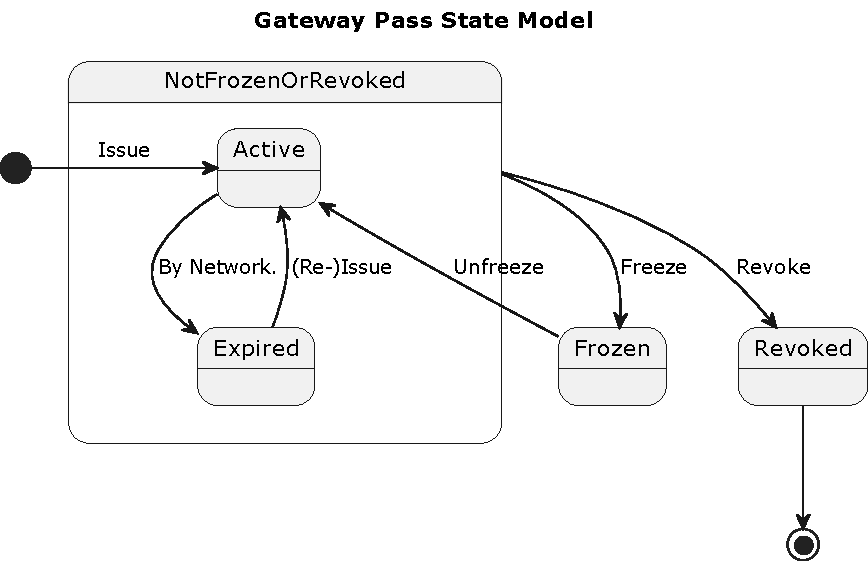
\includegraphics[width=100mm,scale=0.5]{figures/03-pass-state-diagram.pdf}
    \caption[Fig 2]{State Transitions of a Gateway Pass.}
  \end{center}
\end{figure}

\subsection{The Governance Token}
The Gateway Protocol’s native Governance Token is CVC. All Governance Tokens are held and staked on the Solana chain as this is where all governance activities take place.

The Governance Token will be used by two groups:
\begin{enumerate}
\item Ownership of Governance Tokens is a requirement for any individual to become and remain a \textbf{Voter} within the Gateway Protocol. Ownership allows any individual permissionless participation in the Gateway Protocol’s decision processes.
\item Staking Governance Tokens is a requirement for an organization to become and remain a \textbf{Gatekeeper} within any Gatekeeper network. The staking requirement incentivizes Gatekeepers to avoid acting maliciously.
\end{enumerate}

The Governance Token also enables the establishment of a fee structure to fund future protocol development. The Governance Token will not be used to reward any group within the Gateway Protocol—it is purely intended to support governance processes.

